在本实验中, 选取北京, 上海, 广州, 深圳和潍坊五个城市, 借助Scrapy框架设计爬虫, 部
署在Scrapyd上运行爬取; 爬取数据以定义的item结构保存, 通过pipeline传输到使用
SQLite3建立的数据库进行去重, 断点续爬和持久化.

爬虫设置方面, 由于部署在Scrapyd上进行爬取, 因此爬取时间不成为限制. 为了避免可能
出现的反爬措施, 设置下载延迟为6\~10秒, 每个域名并行请求数为2, 每个IP并行请求数为
2, 并使用了轮换的User Agent.

由于链家一次只显示100页, 只有3000个房源, 远小于房源总数, 直接对租房房源进行爬取将遗漏大量房
源信息. 因此为了尽可能多的爬取房源, 制作了三个爬虫, 分别爬取板块(商圈, business
area), 小区(community)和租房房源(rental).在爬取板块的同时, 爬虫可以\textbf{自动
    收集行政区划分}, 小区指北京邮电大学家属小区这一级, 租房房源指具体的出租房源信息.
由于一个小区内不会有超过3000各租房房源,因此通过这一划分方式, 可以尽可能的避免这
一限制造成的爬取不充分. 对三个爬虫分别介绍如下.

\subsection{行政区划和板块爬虫}
这一爬虫是首先运行的爬虫, 定义在 ``business\_area\_spider.py'' 中的
\pythoninline{class BusinessAreaSpider} 中.

其部署到scrapyd或者本地运行后, 将以start\_requests中urls中的url为起点, 对每个城
市的行政区, 以及板块进行爬取.

\subsubsection{爬取结果的持久化}
爬取到的板块将保存在定义在``items.py''中的 \pythoninline{class BusinessAreaItem}
中, 并传输给定义在``pipeline.py''中的 \pythoninline{class
    DownBusinessAreaUrlPipeline} , 由该pipeline判断此BusinessAreaItem所在的城市, 行
政区, 以及此板块是否分别存在与相应数据库表中. 如果不存在, 则插入.

BusinessAreaItem定义如下.
\begin{python}
    class BusinessAreaItem(scrapy.Item):
    # Business area
    business_area_url = scrapy.Field()
    business_area_name = scrapy.Field()
    business_area_region = scrapy.Field()
    business_area_city = scrapy.Field()
\end{python}

分别存储了板块的url, 名称, 行政区和所在城市. 而其保存到的SQL中的板块表还有一个
accessbit字段, 用于判断该板块是否已经被下面介绍的小区爬虫爬取过. 借助这一字段,可
以方便的实现\textbf{断点续爬}: 不会对已经爬取过的小区重复爬取, 而是对因为意外中
断而没有来得及爬取的板块中小区进行爬取.

\subsection{小区爬虫}
这一爬虫在行政区划和板块爬虫爬取完毕后运行, 定义在``community\_spider.py''中的
\pythoninline{class ComemunitySpider(scrapy.Spider)}, 在本地或者scrapyd上启动后,
将首先访问SQLite数据库, 获取没有访问的板块url和对应城市url, 并对其开始并行爬取.
由于小区数量很多, 一页不能完全展示, 所以需要处理\textbf{翻页}问题; 此外, 为了避免对一个区
块的重复爬取, 需要设置\textbf{已爬标记}.

\subsubsection{已爬标记和翻页}
每爬取完一页小区后, 需要借助当前页码和总页数进行判断. 当前页和总页数均存储在
\pythoninline{response.xpath("//div[@class='page-box
house-lst-page-box']/@pagedata")} 中. 如果已经是最后一页小区, 则设置该小区所在的
business\_area的accessbit为1, 表示这一区块已经被爬取过. 如果不是最后一页小区, 则
对response.url进行处理, 提取出当前板块的主url, 并链接
\pythoninline{f"pg{next_page}/"}字段, 作为下一页url进行爬取.

\subsubsection{爬取结果的持久化}
爬取结果保存在\pythoninline{class CommunityItem}中, 传输给
\pythoninline{class DownCommunityInfoPipeline}, 由其根据小区链接
\pythoninline{item["community_url"]} 是否已在数据库中来判断该结果是否重复. 如果
不重复, 则插入数据库. CommunityItem定义如下.
\begin{python}
    class CommunityItem(scrapy.Item):
    # Community
    community_url = scrapy.Field()
    community_name = scrapy.Field()
    community_region = scrapy.Field()
    community_city = scrapy.Field()
    community_business_area = scrapy.Field()
    community_rent_url = scrapy.Field()
\end{python}
分别存储小区链接, 小区名, 小区所在行政区, 小区所在城市, 小区所在板块和小区租房链
接. 其中如果小区内没有房屋出租, 则租房链接为`None', 避免数据库中出现null值.

\subsection{租房房源爬虫}
小区信息爬取完毕后, 在小区信息的基础上进行租房房源信息的爬取. 租房房源爬虫为
``rent\_spider.py''中的 \pythoninline{class RentSpider(scrapy.Spider)}, 首先从数
据库中读取租房链接community\_rent\_url非`None', 且访问位community\_accessbit为0
的小区列表, 再对这些小区进行租房房源的并行爬取. 由于单小区内房源也会有一页不能完
全展示的问题, 因此也需要处理\textbf{翻页}问题. 链家的租房房源不同页的url设计比较
奇怪, 给翻页问题的处理带来了一些困扰.

\subsubsection{已爬标记和翻页}
与爬取板块内小区不同的是, 小区内会出现没有房源正在出租的情况. 通过仔细观察, 注意
到字段 \pythoninline{response.xpath("//span[@class='q']/text())} 记录了当前小区
内房源数量. 如果当前小区内租房房源数量为0, 则设置当前小区的访问位
community\_accessbit为2, 跳过当前小区.

否则, 每爬取完小区内的一页租房房源后, 需要借助当前页码和总页数进行判断. 当前页和
总页数均存储在\pythoninline{response.xpath("//div[@class='content__pg']")} 中.
如果已经是最后一页小区,则设置该页所在小区的community\_accessbit为1, 结束对该小区
的访问.

\subsubsection{爬取结果的持久化}
爬取结果保存在\pythoninline{class RentalItem} 中, 传输给
\pythoninline{class DownRentalInfoPipeline}, 由其根据房源url判断是否已经
在SQLite数据库中的rental表中. 如果不存在, 则插入. RentalItem定义如下:
\begin{python}
    class RentalItem(scrapy.Item):
    # Rental info
    rental_name = scrapy.Field()
    rental_url = scrapy.Field()
    rental_city=scrapy.Field()
    rental_region = scrapy.Field()
    rental_business_area = scrapy.Field()
    rental_community_url=scrapy.Field()
    rental_community = scrapy.Field()
    rental_area = scrapy.Field()
    rental_lighting = scrapy.Field()
    rental_rooms = scrapy.Field()
    rental_liverooms = scrapy.Field()
    rental_bathrooms = scrapy.Field()
    rental_price = scrapy.Field()
    rental_timestamp = scrapy.Field()
\end{python}

\subsection{部署在scrapyd上进行爬取}
完成上述过程后, 为了让爬虫能够稳定运行, 在服务器上安装scrapyd, 部署在端口6800并
转发端口. 在本地使用scrapyd-client将爬虫部署到服务器的scrapyd如图~\ref{fig:运行
在Scrapyd上的爬虫}, 并依次运行BusinessAreaSpider, CommunitySpider和RentSpider进
行爬取.
\begin{figure}[ht!]
    \centering
    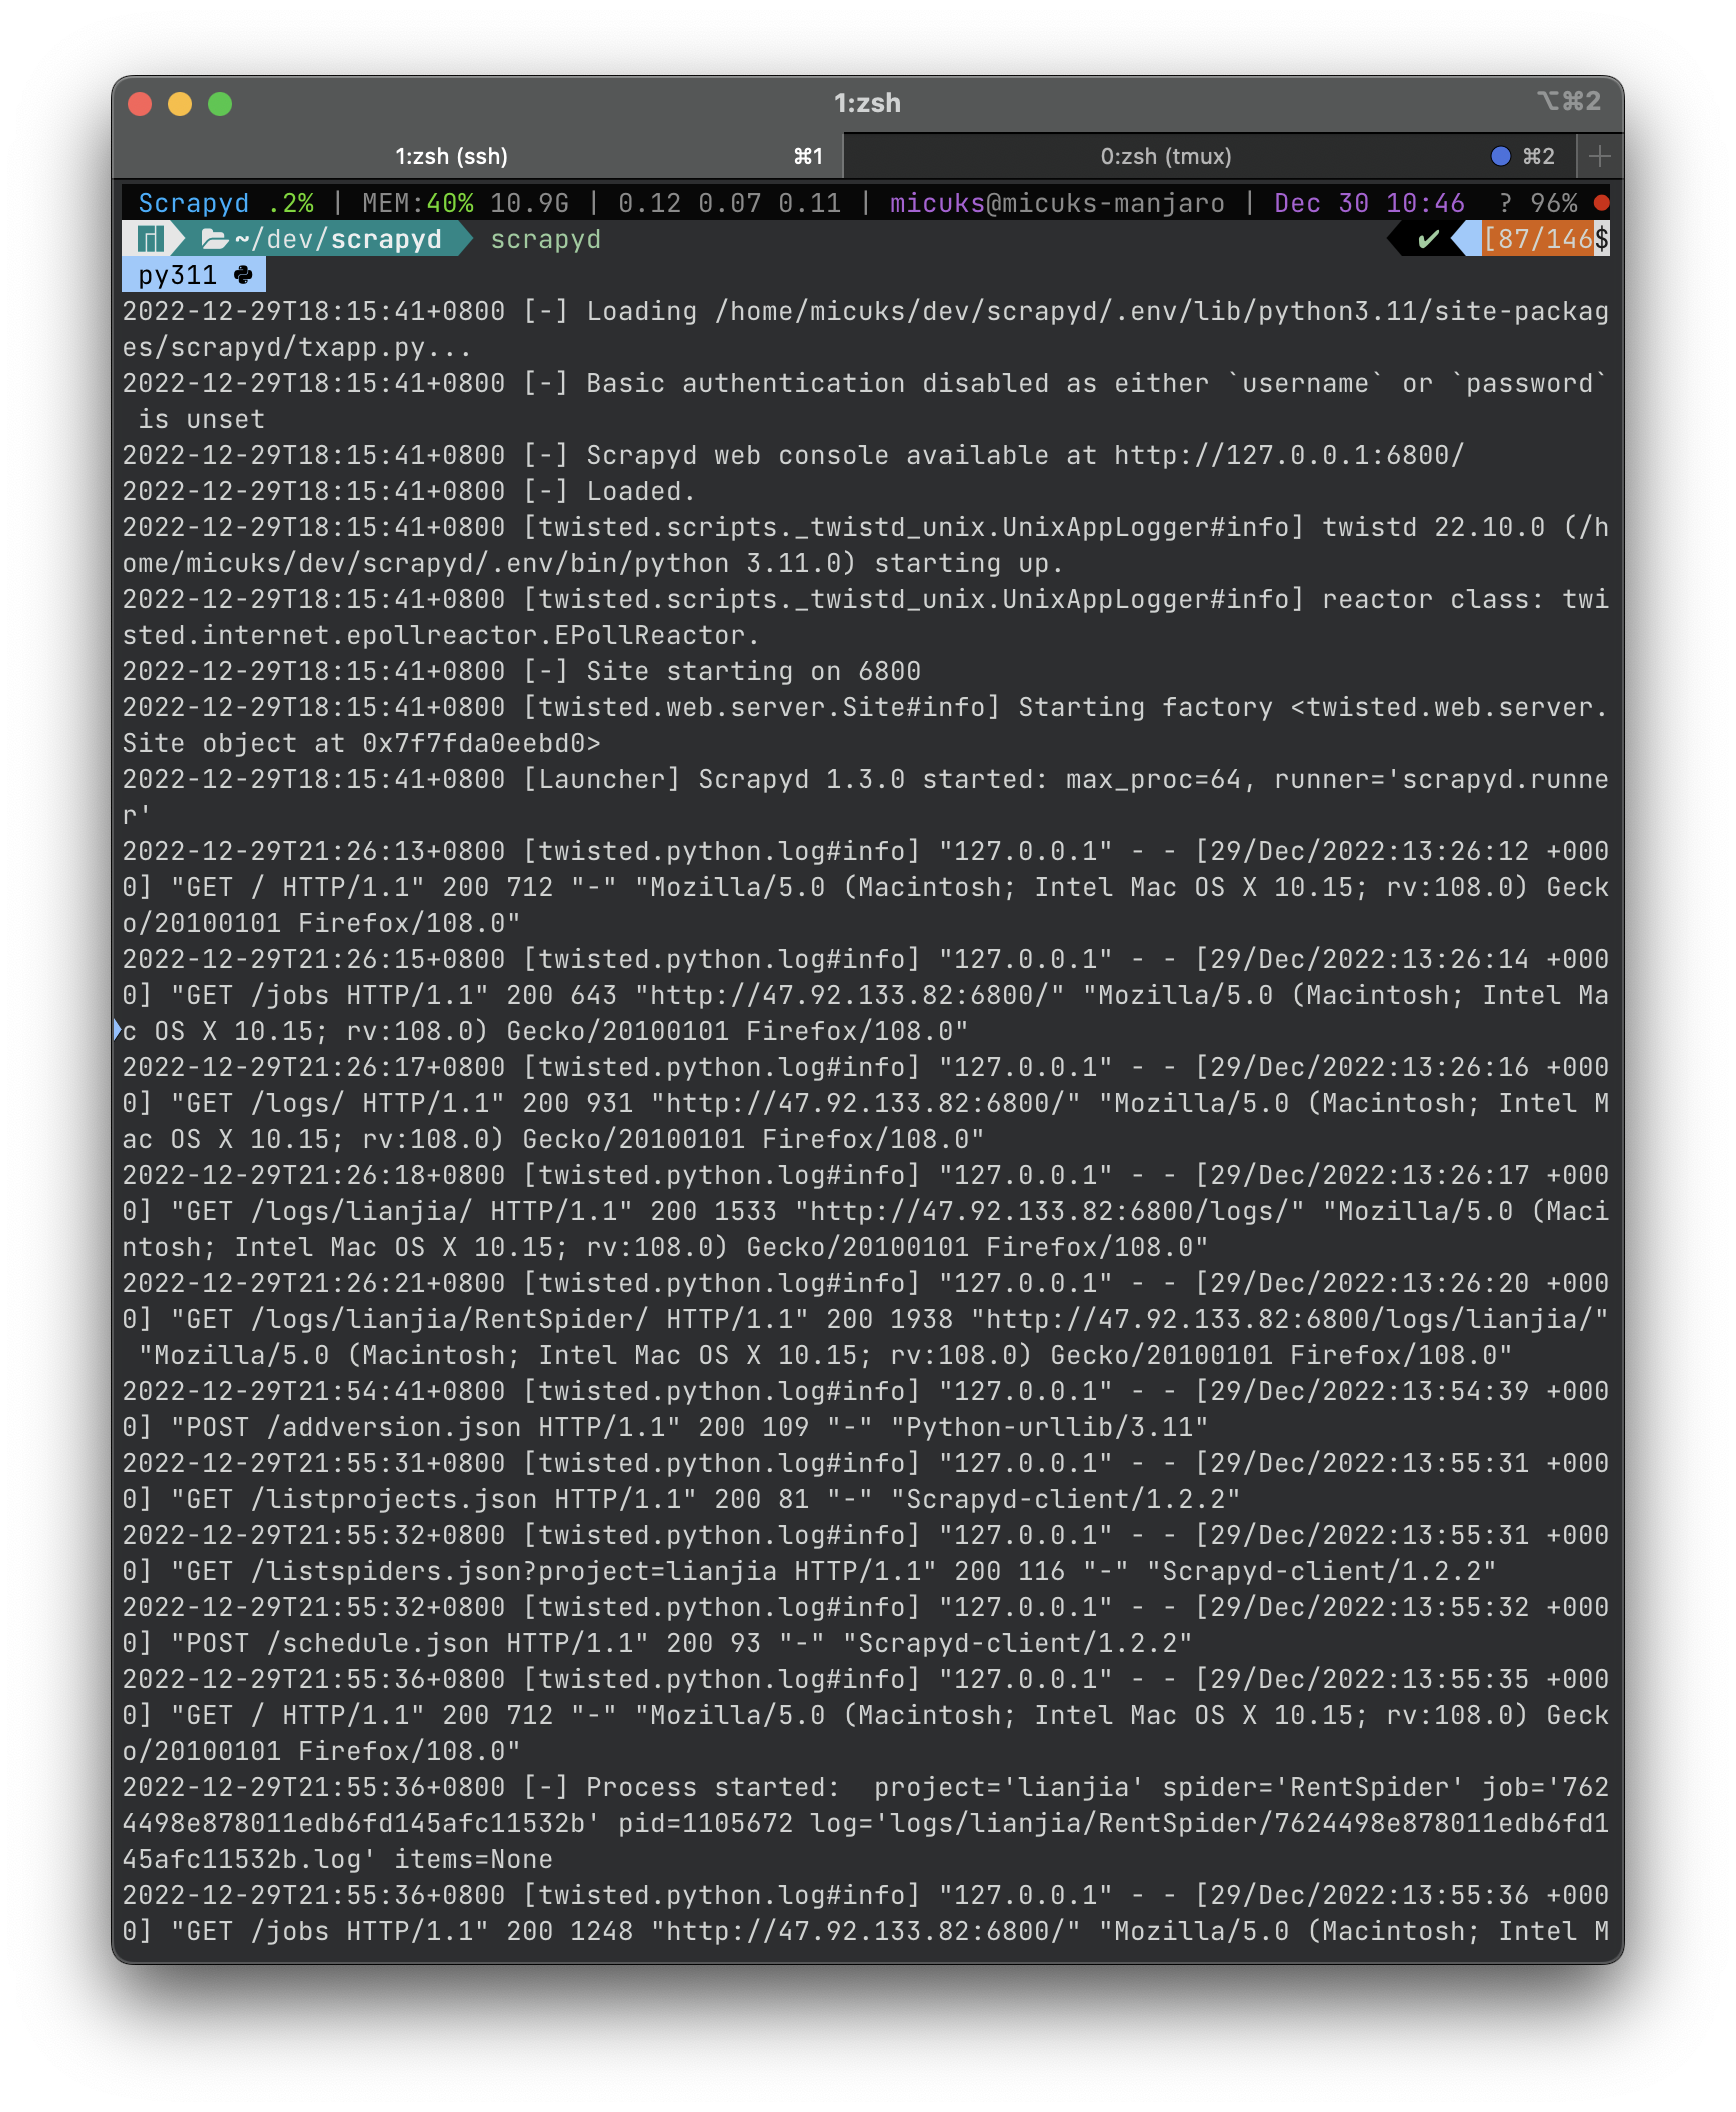
\includegraphics[width=0.95\textwidth]{scrapyd.png}
    \caption{运行在Scrapyd上的爬虫}
    \label{fig:运行在Scrapyd上的爬虫}
\end{figure}